\begin{frame}
\frametitle{Fonction de hachage}


\begin{itemize}
\item A partir d'une donnée fournie en entrée, calcule un haché.\\
\item Résistance au calcul de pré-image.
\item Résistance au calcul de seconde pré-image.
\item Résistance au calcul de collision.\\
\end{itemize}
\end{frame}

\begin{frame}
\frametitle{Présentation MD5}

\begin{itemize}
\item Ronald Rivest en 1991.\\
\item Empreinte est de 128 bits.\\
\item Attaque par collision.
\end{itemize}
\end{frame}

\begin{frame}
\frametitle{schéma Merkle-Damgard}
\begin{figure}[h!]
\center
 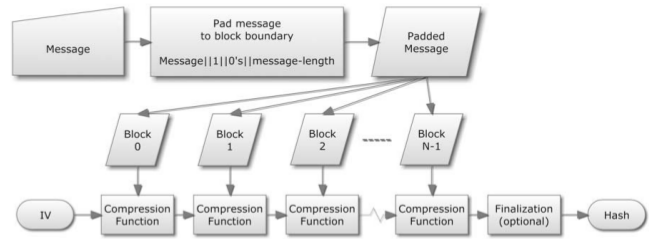
\includegraphics[width=11.5cm]{images/md.png}
 
  \caption{Principe de fonctionnement MD5}
\end{figure}
\end{frame}

\begin{frame}
\frametitle{Fonctionnement MD5}


\begin{itemize}
\item Padding.\\
\item Partitionnement.\\
\item Calcule IHV.\\
\item Le haché.\\

\end{itemize}
\end{frame}


\begin{frame}
\frametitle{Vulnérabilité MD5}

\begin{itemize}
\item Wang et Yu.\\
\item Marc Stevens.\\
\end{itemize}
\end{frame}